\begin{block}{Human Impacts}
    \begin{itemize}
        \item Electricity demand would have broken all-season record \cite{ercotpublic_outagesv1:2021}
        \item Over \SI{30000}{\mega\watt} of lost output (mostly natural gas; see ref.~\cite{ercotpublic_outagesv2:2021})
        \item Grid within minutes of catastrophic failure (\cref{fig:ercot-frequency})
        \item Over 100 people died \cite{mulcahy_urideath:2021}
        \item Estimated \$130 billion damages \cite{busby_cascadingrisks:2021}
        \item Cascading failures of water supply and other critical infrastructure
        \item Marginalized communities disproportionately affected \cite{dobbins_blackoutdisparity:2021}
    \end{itemize}
    \begin{framed}
        \begin{figure}
            \centering
            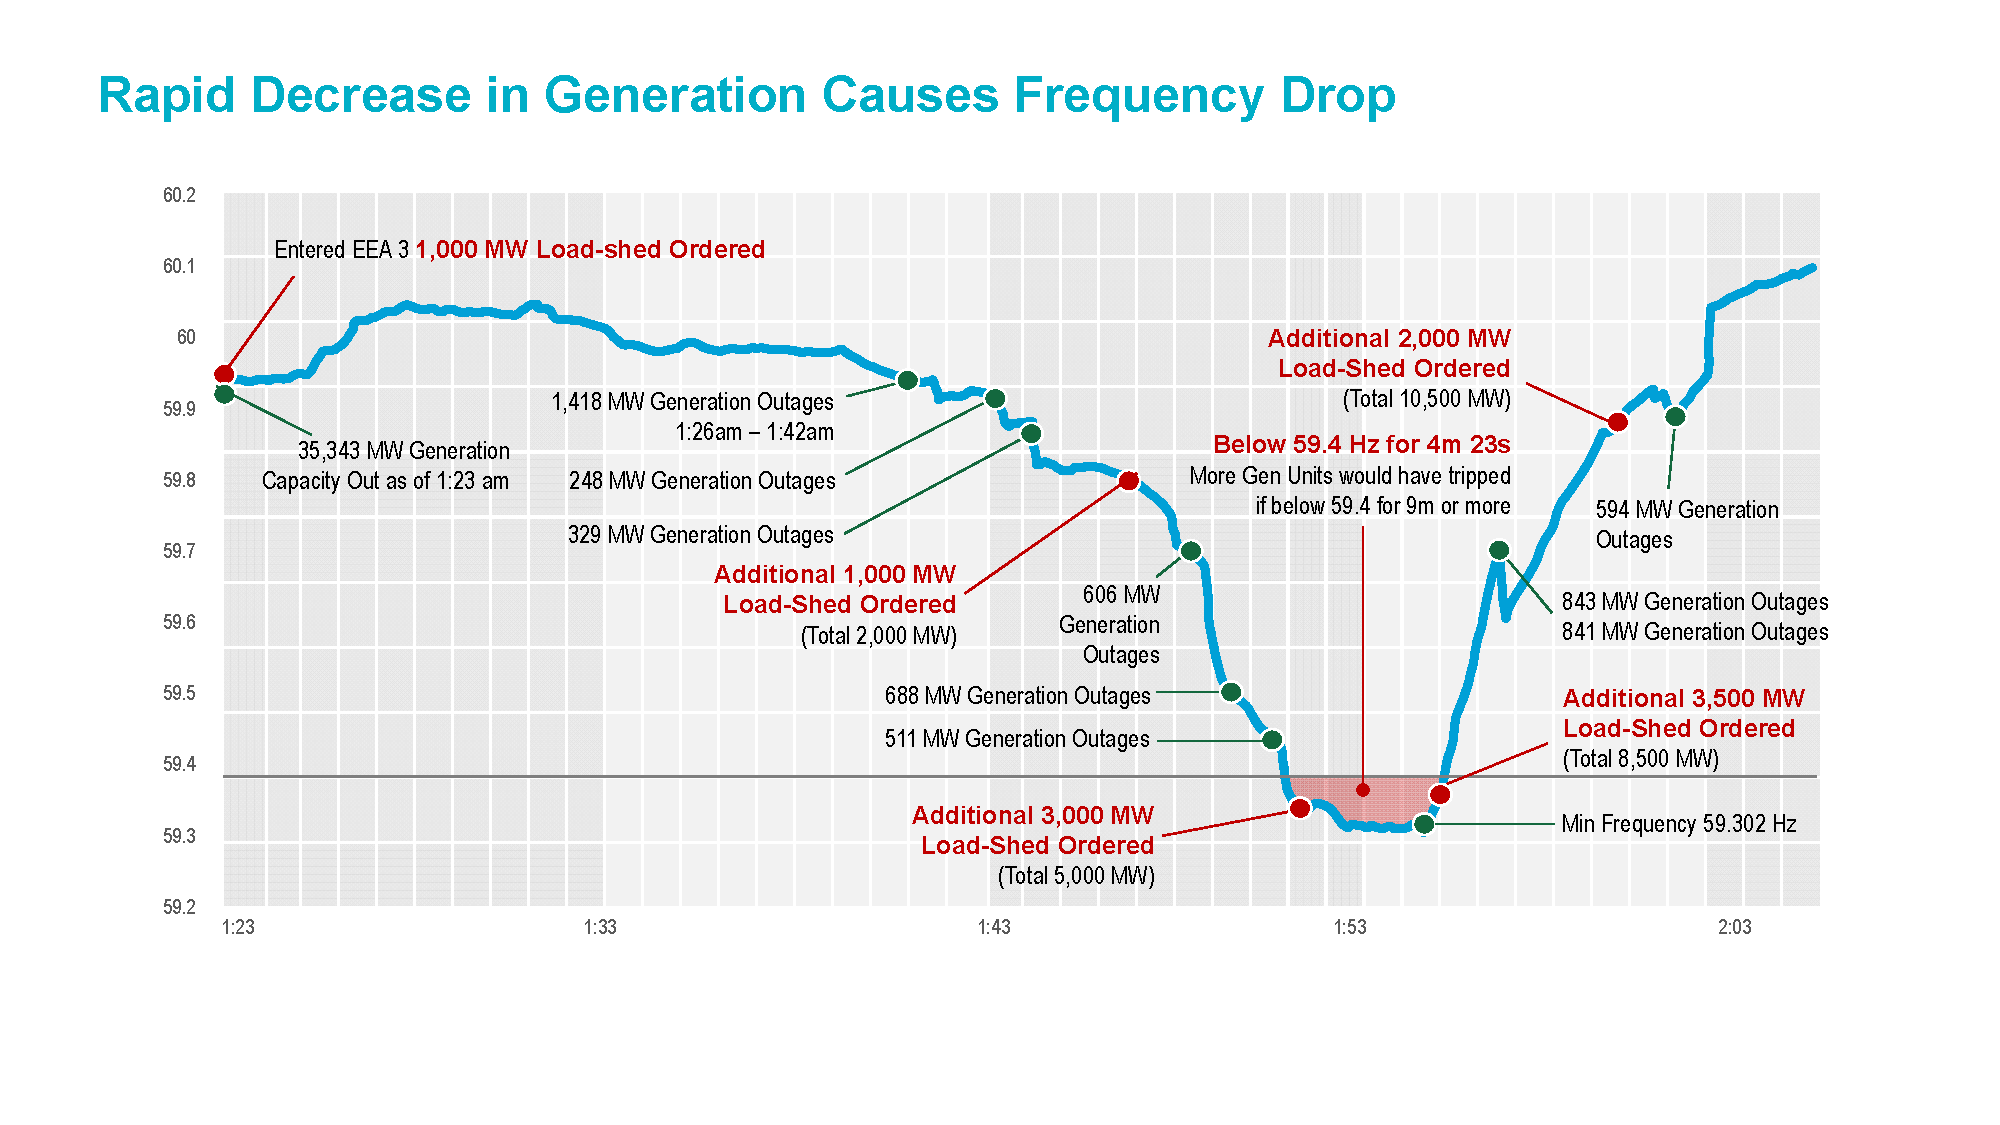
\includegraphics[width=0.8\textwidth]{magness_frequency.pdf}
            \caption{
                As demand spiked and generation failed, the Texas grid came within minutes of catastrophic failure.
                Figure from ERCOT~\cite{magness_review:2021}.
            }
            \label{fig:ercot-frequency}
        \end{figure}
    \end{framed}
\end{block}